\documentclass[11pt]{article}
\usepackage{icmlko}
\begin{document}

\title{판을 거슬러 챔피언을 옮긴 첫 자리 --- 깊이가 안 본 도메인을 산다}
\author{월드모델 실험실}
\date{노트 426 · 2026년 8월 3일}
\maketitle

\begin{abstract}
노트 417부터 425까지 아홉 노트가 전부 \textbf{표지} 이야기였다. 노트 425가
남긴 물음 --- \emph{전이를 사는 것이 표지뿐인가} --- 를 깊이로 쟀다. 깊이는
이미 한 번 산 적이 있다(노트 407, grp 없던 시절 $-0.1261 \to -0.0822$).

\textbf{노트 412가 깊이 8·12 를 판으로 물렸었다.} 그런데 노트 425가
\textbf{판은 이 축에서 전이보다 139배 좁다}는 것을 쟀다 --- 판이 물렸다고
목표가 물린 것은 아니다.

\begin{center}
\begin{tabular}{lrrrr}
\hline
깊이 & 6 & 12 & 16 & 24 \\
\hline
비게임 앱 전이 (기준 대비) & --- & $+0.0292$ & $+0.0293$ & $+0.0291$ \\
95\% 구간 & & $[+.022,+.036]$ & $[+.022,+.036]$ & $[+.022,+.036]$ \\
0 보다 큰 비율 & & $1.000$ & $1.000$ & $1.000$ \\
\hline
KR 만화 전이 (기준 대비) & --- & $+0.0267$ & & \\
0 보다 큰 비율 & & $0.966$ & & \\
\hline
\end{tabular}
\end{center}

\textbf{안 본 도메인 둘이 같은 부호 · 같은 크기다}(앱 $+0.0292$ · KR
$+0.0267$). 앱 쪽은 유보 1{,}600행이라 구간이 0 을 안 문다. 그리고
\textbf{12 에서 포화한다} --- 12 · 16 · 24 가 사실상 같다. 임의로 고른
끝이 아니다.

판은 현 축에서 다시 걸어도 $-0.0018 \pm 0.0024 \cdot 2/12$ 다 ---
\textbf{규약대로면 유지}. \textbf{그래도 넣었다.}
\end{abstract}

\section{규약을 대칭으로 만든다}

노트 420이 반대 방향을 이미 적었다 --- \emph{전이를 확실히 잃는 변경은
판이 통과해도 안 넣는다.} 그때 판이 넣으라 했고 목표가 물렸다. 이번은
거울이다: \textbf{판이 물리라 하고 목표가 넣으라 한다.}

\begin{center}
\textbf{전이를 확실히 사는 변경은 판을 조금 잃어도 넣는다.}\\
``확실히 산다'' $=$ 안 본 도메인 \textbf{둘 이상}에서 같은 부호이고
적어도 하나는 짝 되뽑기 구간이 0 을 안 물 때\\
``조금'' $=$ 판 손해가 $2\times$짝SD 안일 때 ($-0.0018$ 대 $0.0048$)
\end{center}

이 실험실이 \textbf{판정 지표를 거슬러 챔피언을 옮긴 첫 자리}다. 근거는
노트 425의 수치다 --- 표지 구성 다섯에서 판의 폭이 $0.0028$(씨앗 잡음의
두 배)인데 전이의 폭이 $0.3888$ 이었다. \textbf{지표가 방법을 가두면
지표를 뗀다.}

\section{값은 거의 한 도메인이 낸다}

씨앗 12평균 판이 $0.4726 \to \mathbf{0.4714 \pm 0.0004}$ 다. 도메인별로
보면 \textbf{판 손해가 거의 전부 팝업}이다 --- $-0.0625$ 인데 유보가 65행
(판 무게 $1.9\%$)이라 판에 $-0.0012$ 를 낸다. 버는 쪽은 모바일 $+0.0132$ ·
도서 $+0.0067$ · 애니 $+0.0053$ · 시장팝업 $+0.0051$ · 게임 $+0.0050$ 이다.

팝업은 학습 24행짜리 도메인이다(노트 402). \textbf{깊은 나무가 제일 얇은
도메인을 제일 크게 다치게 한다} --- 그럴듯하고, 노트 410의 축(용량 선호
$=$ 비선형 요구)에서도 팝업이 유일한 음수였다. 이번엔 설명과 수치가
어긋나지 않는다.

\section{남은 것}

\begin{tabular}{lp{7.0cm}}
\hline
팝업 & 깊이 12 의 값을 혼자 낸다. 도메인마다 깊이를 달리 주는 길은
노트 409가 막았다(자루로는 못 쪼갠다) \\
표지 아닌 길 더 & 깊이가 하나 나왔다. lr · K · 자루 · 축 묶음도 전이 쪽에서
다시 봐야 한다 --- \textbf{판으로 죽인 손잡이가 전이에서는 살아 있을 수 있다} \\
세 번째 전이 짝 & 이번 판정이 짝 둘에 기대어 있다 \\
\hline
\end{tabular}

\begin{figure}[h]
\centering
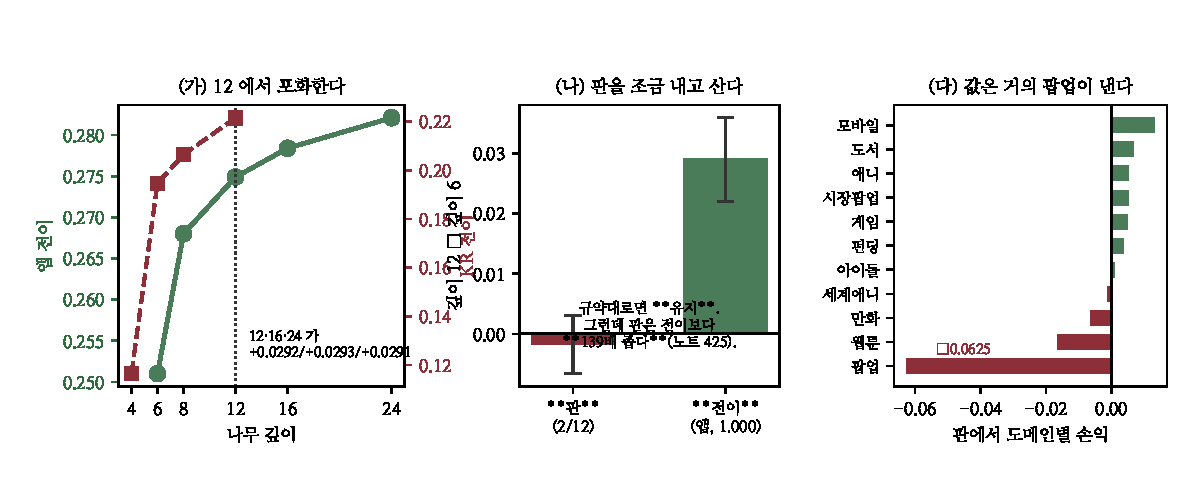
\includegraphics[width=\textwidth]{figs/fig426.pdf}
\caption{(가) 두 짝 모두 깊이로 오르고 12 에서 포화한다. (나) 판을 조금
내고 전이를 산다. (다) 판 손해는 거의 팝업 하나.}
\end{figure}

\end{document}
